Para analizar la calidad del algoritmo realizamos dos tipos diferentes de benchmark, uno que cuantifica la dispersión
media de distintas ejecuciones con distintas semillas para cada algoritmo y otro que estima después de un número
determinado de ejecuciones el tiempo de ejecución medio de cada algoritmo para cada dataset. Cuanto más se aproxime
a cero la dispersión mejor será el algoritmo. A iguales dispersiones consideraremos que un algoritmo es mejor que otro
si el tiempo de ejecución es significativamente menor.

Para el caso de los algoritmos genéticos, a diferencia de para los casos de los algoritmos Greedy y BL, recogeremos 
por cada fichero de benchmark la solución que nos proporcione el algoritmo en cuestión, para una única semilla. Procedemos
de igual forma para el caso de los algoritmos meméticos.

\section{Procedimiento para la obtención de resultados}

Los resultados disponibles en los cuadros de esta sección han sido resultado de distintas ejecuciones.

Para obtener la dispersión hemos ejecutado el algoritmo para cada dataset para 5 semillas distintas disponibles
en el script lanzador. Cada fila de los cuadros 3 y 4 corresponde a la dispersión media de los 5 resultados de cada
una de estas ejecuciones.

Por otra parte, para obtener el tiempo medio de ejecución para fila de las tablas hemos ejecutado cada dataset
para 5 semillas unas 50 veces en invocaciones diferentes y obtenido la media de los resultados del tiempo de estas
$ 50 \cdot 5 $ ejecuciones.

Por último hemos calculado la desviación media de las soluciones para cada tabla como la suma de las desviaciones
entre el número de casos, símil para el caso del cálculo del tiempo medio. La desviación la hemos calculado como la
diferencia entre el coste en dispersión de nuestro algoritmo y el coste de nuestra referencia.

\begin{table}[!ht]%
    \centering
    \begin{tabular}{|l|l|l|}
        \hline
        \textbf{Algoritmo} & \textbf{Desviación~Media} & \textbf{Tiempo~(s)} \\ \hline
        Greedy & 129,45 & 1,53E-03 \\ \hline
        Búsqueda~Local~Primer~Mejor & 87,28 & 1,57E-02 \\ \hline
        Búsqueda~Local & 97,79 & 1,56E-02 \\ \hline
        AGG-uniforme & 77,38 & 5,38E+00 \\ \hline
        AGG-posicion & 92,22 & 1,10E+00 \\ \hline
        AGE-uniforme & 29,88 & 8,81E+00 \\ \hline
        AGE-posicion & 42,15 & 9,54E-01 \\ \hline
        Memetico-10-1.0 & 22,72 & 3,69E+01 \\ \hline
        Memetico-10-0.1 & 42,99 & 3,00E+01 \\ \hline
        Memetico-10-0.1best & 32,94 & 2,97E+01 \\ \hline
    \end{tabular}
\caption{Tabla resumen de las ejecuciones. A menor dispersión mejor resultado.}
\end{table}

\section{Análisis de los datos obtenidos}

En general, los resultados obtenidos son bastante mejorables si los comparamos con las dispersiones de referencia. Como hemos
comentado anteriormente y volveremos a repetir, el factor que más influye en la obtención de resultados es la solución inicial,
ya que al al explorar el espacio de soluciones casi que exclusivamente inmediatamente contiguo será fácil llegar a una solución
la cual no tenga vecinos mejores, quedando por tanto atrapado en un óptimo local y ofreciendo costes muy diferentes según la semilla
utilizada para el generador aleatorio.
Podemos observar estos hechos en la figura 4.1, especialemente en el caso de la Búsqueda Local por Primer Mejor Vecino y por Mejor Vecino.
En general podemos observar que existen muchos resultados con dispersiones muy distintas por encima del tercer cuartil. También lo explicamos
como consecuencia de los factores expuestos.

\begin{figure}[ht]
    \centering
    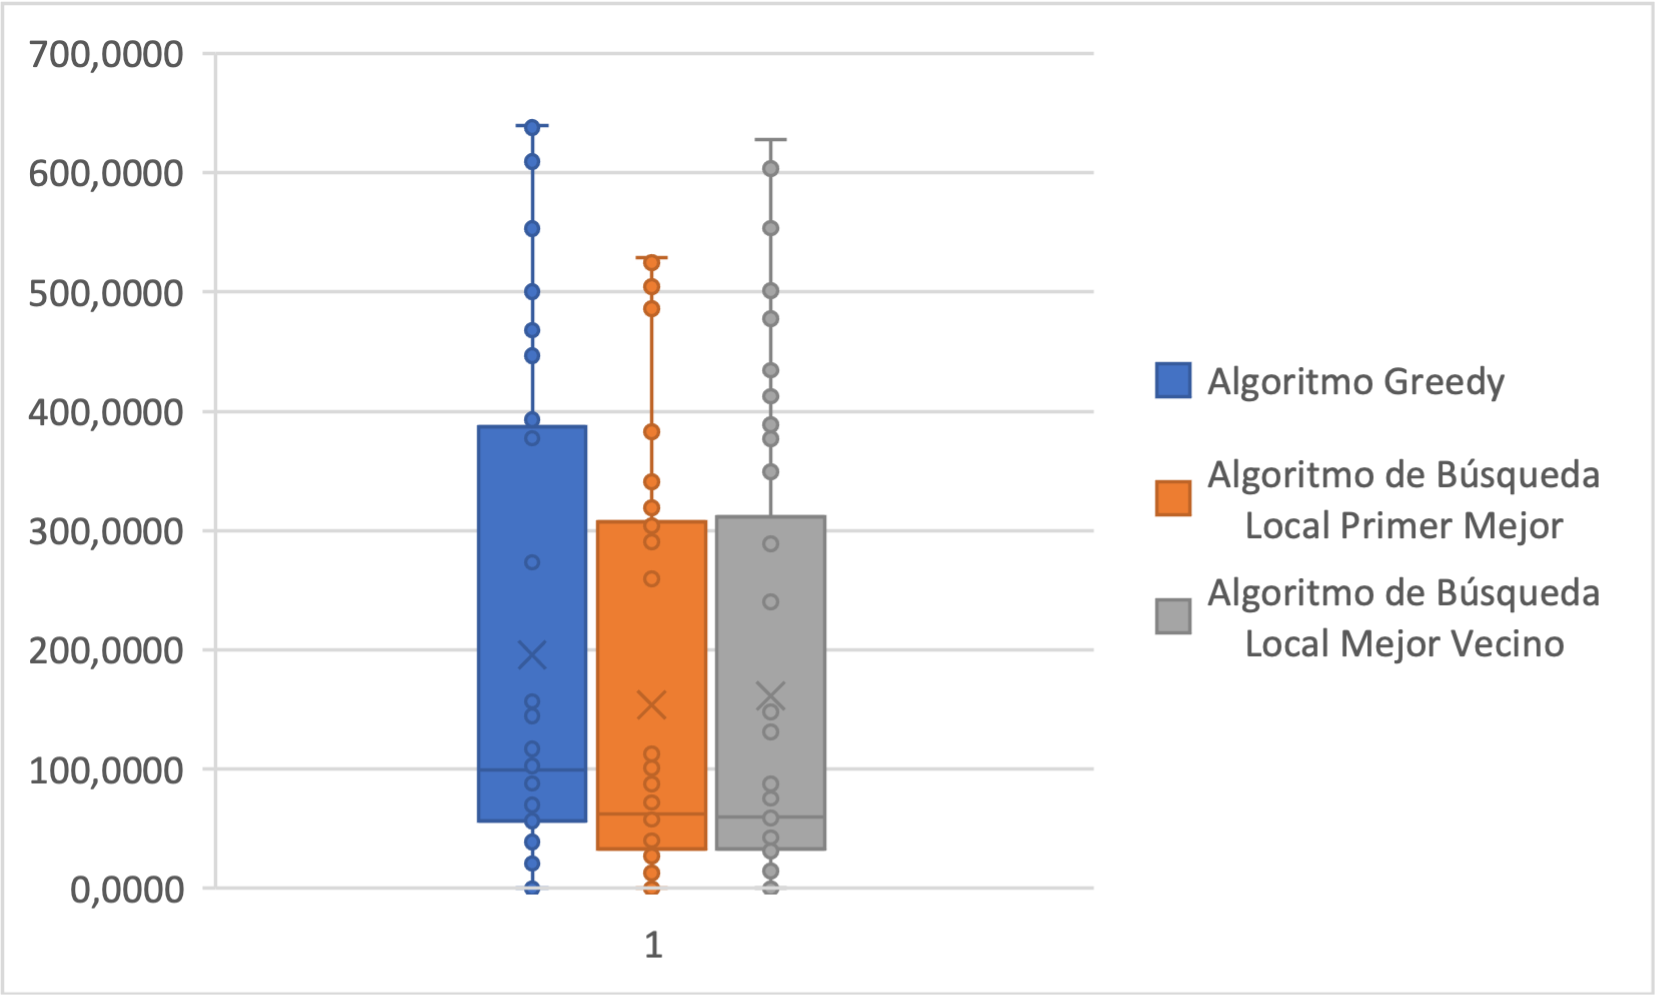
\includegraphics[keepaspectratio]{box_and_whisker_dispersion_media_dataset_y_tipo_algoritmo_greedy_BLPMV_BLMV.png}
    \caption{Dispersión media por dataset y por tipo de algoritmo. Podemos observar que hay una alta desviación típica del coste de las soluciones.
    Destaca el algoritmo de Búsqueda Local por Mejor Vecino por dar peores resultados realizando más iteraciones que el de por Primer
    Mejor Vecino, aunque con mejores resultados de media que el Greedy y con la mediana prácticamente idéntica al Búsqueda Local por Primer Mejor Vecino.
    Esto se debe a que aunque recorre más exhaustivamente el espacio de soluciones y la limitación operador de mutación seguido la BL por Mejor Vecino
    se quede atascado en un óptimo local sin haber explorado mucho el espacio de soluciones, al igual que le ocurre de forma parecida al algoritmo Greedy.}
\end{figure}

Para aumentar el espacio en el espacio de soluciones del conjunto de soluciones consideradas por los algoritmos Greedy y de Búsqueda Local y no quedar
así atrapados en óptimos locales utilizando estrategias de BL podríamos probar variantes como la Búsqueda Local Estocástica, Búsqueda Local por Primer Mejor Aleatorio, Búsqueda Local
con Reinicio Aleatorio u otras técnicas más avanzadas como el Enfriamiento Simulado o búsqueda \textit{Local Beam} entre otros.\cite[Sección 4.1]{russell2020artificial}

\pagebreak

\begin{table}[!ht]%
    \centering    
    \begin{adjustbox}{height=12cm}
    \begin{tabular}{|l|l|l|l|}
    \hline
        Caso & Coste~Medio~Obtenido & Desv & Tiempo~(s) \\ \hline
        GKD-b\_1\_n25\_m2 & 0,0000 & 0,00 & 1,22E-05 \\ \hline
        GKD-b\_2\_n25\_m2 & 0,0000 & 0,00 & 1,36E-05 \\ \hline
        GKD-b\_3\_n25\_m2 & 0,0000 & 0,00 & 1,31E-05 \\ \hline
        GKD-b\_4\_n25\_m2 & 0,0000 & 0,00 & 1,17E-05 \\ \hline
        GKD-b\_5\_n25\_m2 & 0,0000 & 0,00 & 1,14E-05 \\ \hline
        GKD-b\_6\_n25\_m7 & 70,9064 & 58,19 & 5,11E-05 \\ \hline
        GKD-b\_7\_n25\_m7 & 57,0336 & 42,93 & 4,77E-05 \\ \hline
        GKD-b\_8\_n25\_m7 & 44,6512 & 27,89 & 5,08E-05 \\ \hline
        GKD-b\_9\_n25\_m7 & 57,4252 & 40,36 & 5,40E-05 \\ \hline
        GKD-b\_10\_n25\_m7 & 73,3526 & 50,09 & 5,98E-05 \\ \hline
        GKD-b\_11\_n50\_m5 & 20,9113 & 18,99 & 6,85E-05 \\ \hline
        GKD-b\_12\_n50\_m5 & 25,0564 & 22,94 & 7,73E-05 \\ \hline
        GKD-b\_13\_n50\_m5 & 24,8575 & 22,50 & 8,35E-05 \\ \hline
        GKD-b\_14\_n50\_m5 & 30,4310 & 28,77 & 8,29E-05 \\ \hline
        GKD-b\_15\_n50\_m5 & 39,1907 & 36,34 & 8,00E-05 \\ \hline
        GKD-b\_16\_n50\_m15 & 158,8222 & 116,08 & 4,10E-04 \\ \hline
        GKD-b\_17\_n50\_m15 & 150,3960 & 102,29 & 4,11E-04 \\ \hline
        GKD-b\_18\_n50\_m15 & 156,8830 & 113,69 & 4,32E-04 \\ \hline
        GKD-b\_19\_n50\_m15 & 151,8338 & 105,42 & 3,96E-04 \\ \hline
        GKD-b\_20\_n50\_m15 & 145,6224 & 97,91 & 3,48E-04 \\ \hline
        GKD-b\_21\_n100\_m10 & 78,0183 & 64,19 & 3,79E-04 \\ \hline
        GKD-b\_22\_n100\_m10 & 76,9076 & 63,24 & 3,50E-04 \\ \hline
        GKD-b\_23\_n100\_m10 & 81,3711 & 66,03 & 3,44E-04 \\ \hline
        GKD-b\_24\_n100\_m10 & 79,6570 & 71,02 & 3,68E-04 \\ \hline
        GKD-b\_25\_n100\_m10 & 56,6460 & 39,45 & 3,43E-04 \\ \hline
        GKD-b\_26\_n100\_m30 & 377,4836 & 208,75 & 1,98E-03 \\ \hline
        GKD-b\_27\_n100\_m30 & 446,3368 & 319,24 & 2,08E-03 \\ \hline
        GKD-b\_28\_n100\_m30 & 384,7054 & 278,33 & 2,01E-03 \\ \hline
        GKD-b\_29\_n100\_m30 & 273,4050 & 135,95 & 1,98E-03 \\ \hline
        GKD-b\_30\_n100\_m30 & 393,1588 & 265,68 & 2,08E-03 \\ \hline
        GKD-b\_31\_n125\_m12 & 70,1099 & 58,36 & 5,46E-04 \\ \hline
        GKD-b\_32\_n125\_m12 & 89,5372 & 70,75 & 5,56E-04 \\ \hline
        GKD-b\_33\_n125\_m12 & 88,0445 & 69,51 & 5,52E-04 \\ \hline
        GKD-b\_34\_n125\_m12 & 73,3446 & 53,86 & 6,36E-04 \\ \hline
        GKD-b\_35\_n125\_m12 & 95,3074 & 77,19 & 6,45E-04 \\ \hline
        GKD-b\_36\_n125\_m37 & 468,0492 & 312,61 & 3,97E-03 \\ \hline
        GKD-b\_37\_n125\_m37 & 500,5334 & 301,64 & 4,27E-03 \\ \hline
        GKD-b\_38\_n125\_m37 & 553,3864 & 365,42 & 4,17E-03 \\ \hline
        GKD-b\_39\_n125\_m37 & 479,3044 & 310,71 & 4,37E-03 \\ \hline
        GKD-b\_40\_n125\_m37 & 501,5562 & 323,36 & 4,25E-03 \\ \hline
        GKD-b\_41\_n150\_m15 & 113,3785 & 90,03 & 1,14E-03 \\ \hline
        GKD-b\_42\_n150\_m15 & 144,4201 & 117,63 & 1,09E-03 \\ \hline
        GKD-b\_43\_n150\_m15 & 116,8756 & 90,12 & 1,05E-03 \\ \hline
        GKD-b\_44\_n150\_m15 & 109,1999 & 83,26 & 1,04E-03 \\ \hline
        GKD-b\_45\_n150\_m15 & 102,7905 & 75,02 & 1,01E-03 \\ \hline
        GKD-b\_46\_n150\_m45 & 637,9208 & 410,17 & 6,46E-03 \\ \hline
        GKD-b\_47\_n150\_m45 & 477,0816 & 248,48 & 6,39E-03 \\ \hline
        GKD-b\_48\_n150\_m45 & 609,1548 & 382,41 & 6,57E-03 \\ \hline
        GKD-b\_49\_n150\_m45 & 639,2372 & 412,83 & 6,60E-03 \\ \hline
        GKD-b\_50\_n150\_m45 & 471,5032 & 222,65 & 6,38E-03 \\ \hline
    \end{tabular}
    \end{adjustbox}
    \caption{Resultados de la ejecución del algoritmo \textbf{Greedy}}
\end{table}

\pagebreak
\pagebreak

\begin{table}[!ht]
    \centering
    \begin{adjustbox}{height=12cm}
    \begin{tabular}{|l|l|l|l|}
    \hline
        Caso & Coste medio obtenido & Desv & Tiempo~(s) \\ \hline
        GKD-b\_1\_n25\_m2 & 0,0000 & 0,00 & 1,86E-05 \\ \hline
        GKD-b\_2\_n25\_m2 & 0,0000 & 0,00 & 1,70E-05 \\ \hline
        GKD-b\_3\_n25\_m2 & 0,0000 & 0,00 & 1,89E-05 \\ \hline
        GKD-b\_4\_n25\_m2 & 0,0000 & 0,00 & 1,76E-05 \\ \hline
        GKD-b\_5\_n25\_m2 & 0,0000 & 0,00 & 1,72E-05 \\ \hline
        GKD-b\_6\_n25\_m7 & 30,5731 & 17,86 & 2,73E-04 \\ \hline
        GKD-b\_7\_n25\_m7 & 27,2974 & 13,20 & 2,16E-04 \\ \hline
        GKD-b\_8\_n25\_m7 & 42,2687 & 25,51 & 2,41E-04 \\ \hline
        GKD-b\_9\_n25\_m7 & 40,2675 & 23,20 & 2,42E-04 \\ \hline
        GKD-b\_10\_n25\_m7 & 45,7940 & 22,53 & 2,23E-04 \\ \hline
        GKD-b\_11\_n50\_m5 & 15,5196 & 13,59 & 2,80E-04 \\ \hline
        GKD-b\_12\_n50\_m5 & 11,3000 & 9,18 & 2,35E-04 \\ \hline
        GKD-b\_13\_n50\_m5 & 13,1555 & 10,79 & 2,84E-04 \\ \hline
        GKD-b\_14\_n50\_m5 & 21,0886 & 19,43 & 2,26E-04 \\ \hline
        GKD-b\_15\_n50\_m5 & 17,2445 & 14,39 & 2,65E-04 \\ \hline
        GKD-b\_16\_n50\_m15 & 100,7846 & 58,04 & 2,99E-03 \\ \hline
        GKD-b\_17\_n50\_m15 & 115,8601 & 67,75 & 3,04E-03 \\ \hline
        GKD-b\_18\_n50\_m15 & 87,7141 & 44,52 & 2,18E-03 \\ \hline
        GKD-b\_19\_n50\_m15 & 110,8314 & 64,42 & 2,26E-03 \\ \hline
        GKD-b\_20\_n50\_m15 & 112,7244 & 65,01 & 2,84E-03 \\ \hline
        GKD-b\_21\_n100\_m10 & 33,8073 & 19,98 & 2,09E-03 \\ \hline
        GKD-b\_22\_n100\_m10 & 47,3694 & 33,71 & 1,76E-03 \\ \hline
        GKD-b\_23\_n100\_m10 & 38,7309 & 23,39 & 1,94E-03 \\ \hline
        GKD-b\_24\_n100\_m10 & 37,8747 & 29,23 & 2,02E-03 \\ \hline
        GKD-b\_25\_n100\_m10 & 36,5649 & 19,36 & 1,96E-03 \\ \hline
        GKD-b\_26\_n100\_m30 & 383,0796 & 214,35 & 1,40E-02 \\ \hline
        GKD-b\_27\_n100\_m30 & 319,3224 & 192,23 & 2,10E-02 \\ \hline
        GKD-b\_28\_n100\_m30 & 259,7818 & 153,40 & 2,38E-02 \\ \hline
        GKD-b\_29\_n100\_m30 & 290,5872 & 153,13 & 2,09E-02 \\ \hline
        GKD-b\_30\_n100\_m30 & 303,7936 & 176,31 & 1,95E-02 \\ \hline
        GKD-b\_31\_n125\_m12 & 48,1569 & 36,41 & 3,34E-03 \\ \hline
        GKD-b\_32\_n125\_m12 & 47,2372 & 28,45 & 3,30E-03 \\ \hline
        GKD-b\_33\_n125\_m12 & 43,2685 & 24,74 & 3,68E-03 \\ \hline
        GKD-b\_34\_n125\_m12 & 48,4522 & 28,96 & 3,77E-03 \\ \hline
        GKD-b\_35\_n125\_m12 & 57,8748 & 39,76 & 3,19E-03 \\ \hline
        GKD-b\_36\_n125\_m37 & 341,0166 & 185,58 & 4,36E-02 \\ \hline
        GKD-b\_37\_n125\_m37 & 524,9386 & 326,04 & 4,93E-02 \\ \hline
        GKD-b\_38\_n125\_m37 & 514,5118 & 326,54 & 4,93E-02 \\ \hline
        GKD-b\_39\_n125\_m37 & 352,4736 & 183,88 & 2,90E-02 \\ \hline
        GKD-b\_40\_n125\_m37 & 388,1836 & 209,99 & 3,89E-02 \\ \hline
        GKD-b\_41\_n150\_m15 & 66,5911 & 43,25 & 7,64E-03 \\ \hline
        GKD-b\_42\_n150\_m15 & 72,0939 & 45,30 & 9,57E-03 \\ \hline
        GKD-b\_43\_n150\_m15 & 75,4758 & 48,72 & 1,07E-02 \\ \hline
        GKD-b\_44\_n150\_m15 & 68,2100 & 42,27 & 7,63E-03 \\ \hline
        GKD-b\_45\_n150\_m15 & 68,9531 & 41,18 & 6,29E-03 \\ \hline
        GKD-b\_46\_n150\_m45 & 529,0926 & 301,34 & 9,12E-02 \\ \hline
        GKD-b\_47\_n150\_m45 & 393,5756 & 164,97 & 7,03E-02 \\ \hline
        GKD-b\_48\_n150\_m45 & 485,8222 & 259,08 & 8,67E-02 \\ \hline
        GKD-b\_49\_n150\_m45 & 504,2588 & 277,85 & 6,70E-02 \\ \hline
        GKD-b\_50\_n150\_m45 & 513,8540 & 265,00 & 7,62E-02 \\ \hline
    \end{tabular}
    \end{adjustbox}
    \caption{Resultados de la ejecución del algoritmo de \textbf{Búsqueda Local Primero el Mejor}}
\end{table}

\pagebreak
\pagebreak

\begin{table}[!ht]
    \centering
    \begin{adjustbox}{height=12cm}
    \begin{tabular}{|l|l|l|l|}
    \hline
        Caso & Coste medio obtenido & Desv & Tiempo~(s) \\ \hline
        GKD-b\_1\_n25\_m2    & 0,0000   & 0,00   & 1,48E-05 \\ \hline
        GKD-b\_2\_n25\_m2    & 0,0000   & 0,00   & 1,47E-05 \\ \hline
        GKD-b\_3\_n25\_m2    & 0,0000   & 0,00   & 1,43E-05 \\ \hline
        GKD-b\_4\_n25\_m2    & 0,0000   & 0,00   & 1,46E-05 \\ \hline
        GKD-b\_5\_n25\_m2    & 0,0000   & 0,00   & 1,43E-05 \\ \hline
        GKD-b\_6\_n25\_m7    & 41,0147  & 28,30  & 2,47E-04 \\ \hline
        GKD-b\_7\_n25\_m7    & 31,2380  & 17,14  & 2,05E-04 \\ \hline
        GKD-b\_8\_n25\_m7    & 39,7308  & 22,97  & 2,85E-04 \\ \hline
        GKD-b\_9\_n25\_m7    & 31,4245  & 14,36  & 2,33E-04 \\ \hline
        GKD-b\_10\_n25\_m7   & 41,0366  & 17,77  & 2,00E-04 \\ \hline
        GKD-b\_11\_n50\_m5   & 14,5492  & 12,62  & 2,25E-04 \\ \hline
        GKD-b\_12\_n50\_m5   & 14,5271  & 12,41  & 2,68E-04 \\ \hline
        GKD-b\_13\_n50\_m5   & 16,6929  & 14,33  & 3,07E-04 \\ \hline
        GKD-b\_14\_n50\_m5   & 18,1709  & 16,51  & 2,26E-04 \\ \hline
        GKD-b\_15\_n50\_m5   & 17,6994  & 14,85  & 2,93E-04 \\ \hline
        GKD-b\_16\_n50\_m15  & 133,7260 & 90,98  & 2,28E-03 \\ \hline
        GKD-b\_17\_n50\_m15  & 94,6846  & 46,58  & 2,52E-03 \\ \hline
        GKD-b\_18\_n50\_m15  & 87,7548  & 44,56  & 2,58E-03 \\ \hline
        GKD-b\_19\_n50\_m15  & 147,9698 & 101,56 & 2,43E-03 \\ \hline
        GKD-b\_20\_n50\_m15  & 131,2973 & 83,58  & 2,01E-03 \\ \hline
        GKD-b\_21\_n100\_m10 & 34,1728  & 20,34  & 2,34E-03 \\ \hline
        GKD-b\_22\_n100\_m10 & 47,1748  & 33,51  & 2,04E-03 \\ \hline
        GKD-b\_23\_n100\_m10 & 44,0858  & 28,74  & 2,20E-03 \\ \hline
        GKD-b\_24\_n100\_m10 & 39,6790  & 31,04  & 2,36E-03 \\ \hline
        GKD-b\_25\_n100\_m10 & 40,9679  & 23,77  & 2,17E-03 \\ \hline
        GKD-b\_26\_n100\_m30 & 289,2192 & 120,49 & 2,19E-02 \\ \hline
        GKD-b\_27\_n100\_m30 & 240,0852 & 112,99 & 1,75E-02 \\ \hline
        GKD-b\_28\_n100\_m30 & 298,6812 & 192,30 & 1,76E-02 \\ \hline
        GKD-b\_29\_n100\_m30 & 349,2608 & 211,81 & 2,55E-02 \\ \hline
        GKD-b\_30\_n100\_m30 & 360,5168 & 233,04 & 1,81E-02 \\ \hline
        GKD-b\_31\_n125\_m12 & 53,0276  & 41,28  & 5,34E-03 \\ \hline
        GKD-b\_32\_n125\_m12 & 53,3928  & 34,60  & 4,12E-03 \\ \hline
        GKD-b\_33\_n125\_m12 & 70,1904  & 51,66  & 4,31E-03 \\ \hline
        GKD-b\_34\_n125\_m12 & 42,8187  & 23,33  & 4,10E-03 \\ \hline
        GKD-b\_35\_n125\_m12 & 58,9108  & 40,80  & 4,51E-03 \\ \hline
        GKD-b\_36\_n125\_m37 & 377,0292 & 221,59 & 4,29E-02 \\ \hline
        GKD-b\_37\_n125\_m37 & 388,9456 & 190,05 & 4,08E-02 \\ \hline
        GKD-b\_38\_n125\_m37 & 479,3834 & 291,42 & 4,44E-02 \\ \hline
        GKD-b\_39\_n125\_m37 & 412,7346 & 244,14 & 4,31E-02 \\ \hline
        GKD-b\_40\_n125\_m37 & 501,2238 & 323,03 & 3,84E-02 \\ \hline
        GKD-b\_41\_n150\_m15 & 52,4719  & 29,13  & 6,65E-03 \\ \hline
        GKD-b\_42\_n150\_m15 & 75,4492  & 48,66  & 8,16E-03 \\ \hline
        GKD-b\_43\_n150\_m15 & 61,8164  & 35,06  & 9,66E-03 \\ \hline
        GKD-b\_44\_n150\_m15 & 69,7760  & 43,84  & 8,68E-03 \\ \hline
        GKD-b\_45\_n150\_m15 & 63,4787  & 35,71  & 8,03E-03 \\ \hline
        GKD-b\_46\_n150\_m45 & 628,0786 & 400,33 & 7,43E-02 \\ \hline
        GKD-b\_47\_n150\_m45 & 434,5290 & 205,93 & 7,39E-02 \\ \hline
        GKD-b\_48\_n150\_m45 & 477,4856 & 250,74 & 5,92E-02 \\ \hline
        GKD-b\_49\_n150\_m45 & 603,2906 & 376,88 & 9,15E-02 \\ \hline
        GKD-b\_50\_n150\_m45 & 553,6642 & 304,81 & 8,04E-02 \\ \hline
    \end{tabular}
    \end{adjustbox}
    \caption{Resultados de la ejecución del algoritmo de \textbf{Búsqueda Local}}
\end{table}

\pagebreak